\documentclass[fleqn, xcolor=x11names]{beamer}
\usetheme{Ann}
\usecolortheme{default}

\usepackage[utf8]{inputenc}
\usepackage[T2A]{fontenc}
\usepackage[russian]{babel}
\usepackage{amsmath}
\usepackage{amsfonts}
%\usepackage{amssymb}
\usepackage{hyperref}


\usepackage{graphics, graphicx}
\usepackage{color}
\usepackage{enumerate}

\usepackage{epigraph}
\usepackage{makecell}

\usepackage{tikz}
\usetikzlibrary{patterns}

\usepackage{minted}
\usemintedstyle{default}
%my package
\graphicspath{{../figures/}}
\setbeamertemplate{bibliography item}{\insertbiblabel}

\beamertemplatenavigationsymbolsempty

\setbeamertemplate{itemize item}[ball]
\setbeamertemplate{itemize subitem}[ball]
\definecolor{my_blue}{RGB}{0, 0, 100}


%\usefonttheme[onlylarge]{structurebold} % названия и текст в колонтитулах выводится полужирным шрифтом.
\usefonttheme[onlymath]{serif}  % привычный шрифт для математических формул
%\setbeamerfont*{frametitle}{size=\normalsize,series=\bfseries} % шрифт заголовков слайдов
\usepackage[nopar]{lipsum} %для генерации большого текста

\newminted[pcode]{python}{baselinestretch=1, fontsize=\small}
\newmintinline[pinline]{python3}{baselinestretch=1}
%\definecolor{bg}{rgb}{0.95,0.95,0.95}
%\newminted[lcode]{latex}{baselinestretch=1, bgcolor=bg}
\newmintinline[linline]{latex}{baselinestretch=1}

\usepackage{tcolorbox}
\tcbuselibrary{minted,skins}

\newtcblisting{lcode}{
    listing engine=minted, %use minted for highlight
    colback=lcodebg, %background color
    colframe=black!50, %width of frame
    listing only,
    minted style=colorful,
    minted language=latex,
    minted options={linenos=false,texcl=true}, %lines - number of lines
    left=1mm,
}
\definecolor{lcodebg}{rgb}{0.95,0.95,0.95}

\usepackage{tikz}
\usetikzlibrary{arrows,positioning}
\usepackage{listings}
\lstset{language=Python}

\newcommand{\real}{\mathbb{R}}
\newcommand{\norm}{\mathop{\rm norm}\limits}
\newcommand{\softmax}{\mathop{\rm softmax}\limits}
\newcommand{\argmin}{\mathop{\rm argmin}\limits}

\definecolor{beamer@blendedblue}{rgb}{0.037,0.366,0.75}

\title{\bfseries Распознавание и генерация изображений рукописных текстов на русском языке}
\author[Тыцкий В.И.]{Студент: Тыцкий В.И. \\[1ex]  {\small Научный руководитель: Майсурадзе А.И.}}
\institute[ВМК МГУ]{МГУ имени М. В. Ломоносова, факультет ВМК, кафедра ММП}
\date{}

\begin{document}

\begin{frame}
    \titlepage
\end{frame}

% \begin{frame}{Оглавление}
%      \tableofcontents
% \end{frame}


% \section{Введение}

\begin{frame}{Введение}
    \begin{itemize}
        \item Распознавание текста (OCR) важная задача в машинном обучении
        \item Распознавание \textbf{печатного текста} решается достаточно хорошо
        \item Рукописные тексты обладают большей спецификой
        \begin{itemize}
            \item Малое количество данных
            \item Более сложный домен -- каждый почерк уникален
        \end{itemize}
    \end{itemize}
    
\end{frame}

% \section{Обзор}

\begin{frame}{Данные}
    
    \begin{itemize}
        \item Cyrillic Handwriting Dataset (CyrHD)  \cite{chd}
        \item Handwritten Kazakh and Russian (HKR) (не для коммерческого использования)  \cite{hkr}
        \item IAM Handwriting Database \cite{iam}
    \end{itemize}

    \vspace{10pt}
    \textbf{Принято решение собрать свой датасет}
    
\end{frame}


\begin{frame}{Связанные работы}
    \begin{itemize}
        \item Attention-based Fully Gated for Russian Handwritten Text \cite{CNN-BGRU}
        \item Scrabblegan: Semi-supervised varying length handwritten text generation \cite{scrabble_gan}
    \end{itemize}

\end{frame}



% \section{Актуальность}

\begin{frame}{Актуальность}
    \begin{itemize}
        \item Модель русского рукописного распознавания может использоваться
        в индустрии
        \item Собранные данные могут быть полезны для сообщества
        \item Генерация синтетических данных GAN'ом может применяться
        для создания правдоподобных рукописных текстов
    \end{itemize}
\end{frame}

% \section{Постановка задачи}

\begin{frame}{Постановка задачи}
    \begin{itemize}
        \item Собрать данные с помощью краудфандинга 
        \item Обучить нейронную сеть для распознавания
        русских рукописных текстов
        \item Попробовать использовать синтетические данные, 
        сгенерированные GAN'ом для улучшения качества распознавания

    \end{itemize}
\end{frame}

% \section{Процесс решения}

\begin{frame}{Сбор данных}
    \begin{itemize}
        \item Сбор данных проводился в сервисе Толока
        \item Людей просили написать короткую строчку заранее заданного русского текста
        \item Проверка корректности внесенных изображений проводилась голосованием с перекрытием
        \item Данные можно использовать как для обучения распознавания, так и для обучения GAN'а
    \end{itemize}

    \vspace{10pt}


\end{frame}

\begin{frame}{Обучение модели}
    \centering
    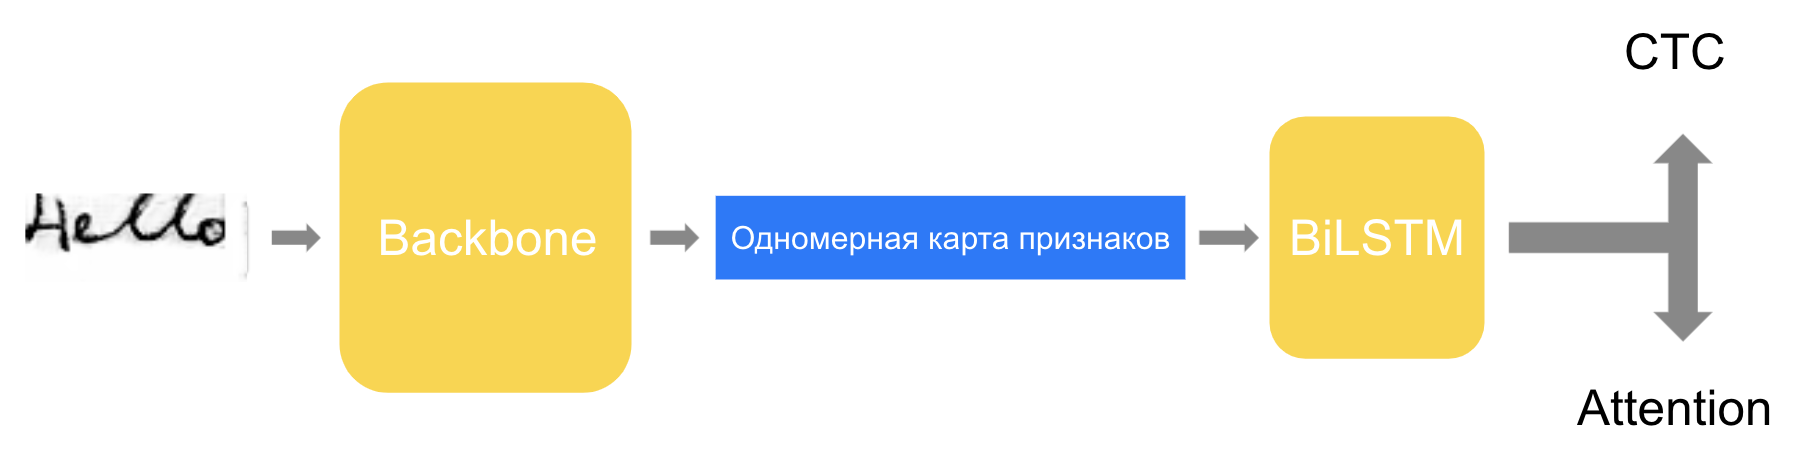
\includegraphics[width=0.8\linewidth]{recognition.png}
    \begin{itemize}
        \item backbone: Inception 
        \item BiLSTM: 512 hidden size
        \item Выход: train -- Attention + CTC, eval -- CTC
    \end{itemize}
\end{frame}

\begin{frame}{Синтетика GAN'ом}

    \begin{columns}
        \begin{column}{0.4\textwidth}
            За основу взят Scrabble GAN \cite{scrabble_gan}
        \end{column}
        \begin{column}{0.6\textwidth}  %%<--- here
            \centering
            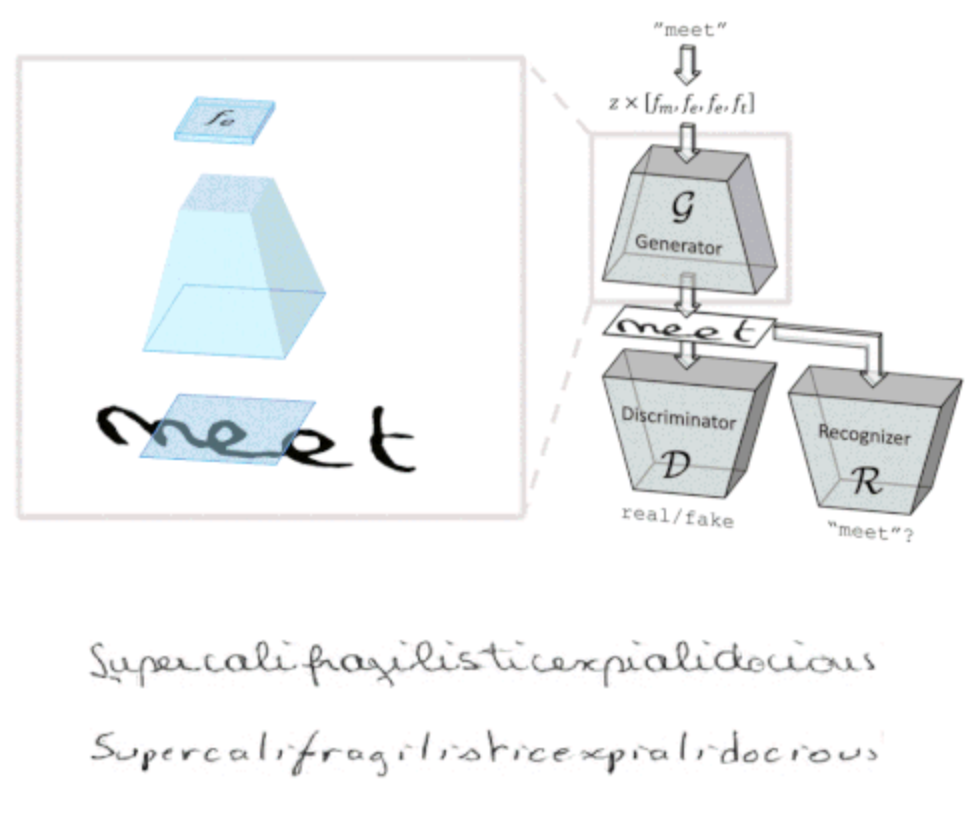
\includegraphics[width=\linewidth]{scrabble_gan.png}
        \end{column}
    \end{columns}
    
\end{frame}

% \section{Результаты}

\begin{frame}{Данные}

    \begin{columns}
        \begin{column}{0.45\textwidth}
            \begin{itemize}
                \item Легко масштабируемый процесс сбора
                \item Размер датасета: 13000 строк
                \item ''Некачественных'' данных < 4\% 
            \end{itemize}
        \end{column}
        \begin{column}{0.55\textwidth}  %%<--- here
            \centering
            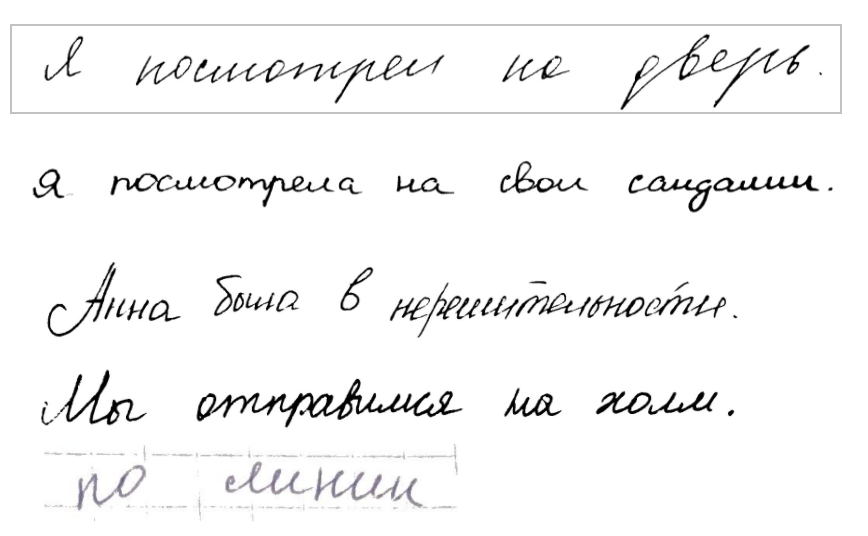
\includegraphics[width=\linewidth]{RHD.png}
        \end{column}
    \end{columns}
\end{frame}

\begin{frame}{Модель}
    \begin{table}[]
        \begin{tabular}{|l|cc|cc|cc|}
        \hline
        \textbf{Data}          & \multicolumn{2}{l|}{\textbf{RHD (ours)}}                              & \multicolumn{2}{l|}{\textbf{CyHD}}                                     & \multicolumn{2}{l|}{\textbf{IAM (EN)}}                                 \\ \hline
        \textbf{}              & \multicolumn{1}{l|}{\textbf{WER}} & \multicolumn{1}{l|}{\textbf{CER}} & \multicolumn{1}{l|}{\textbf{WER}}  & \multicolumn{1}{l|}{\textbf{CER}} & \multicolumn{1}{l|}{\textbf{WER}}  & \multicolumn{1}{l|}{\textbf{CER}} \\ \hline
        \textit{\textbf{Ours}} & \multicolumn{1}{c|}{0.09}         & 0.04                              & \multicolumn{1}{c|}{\textbf{0.39}} & \textbf{0.11}                     & \multicolumn{1}{c|}{\textbf{0.21}} & \textbf{0.08}                     \\ \hline
        CNN-BGRU               & \multicolumn{1}{c|}{-}            & -                                 & \multicolumn{1}{c|}{-}             & -                                 & \multicolumn{1}{c|}{0.25}          & 0.08                              \\ \hline
        Kaggle                 & \multicolumn{1}{c|}{-}            & -                                 & \multicolumn{1}{c|}{0.50}          & 0.11                              & \multicolumn{1}{c|}{-}             & -                                 \\ \hline
        \end{tabular}
    \end{table}
    
\end{frame}


\begin{frame}{Синтетика GAN'ом}
    EN
    \begin{figure}
        \centering
        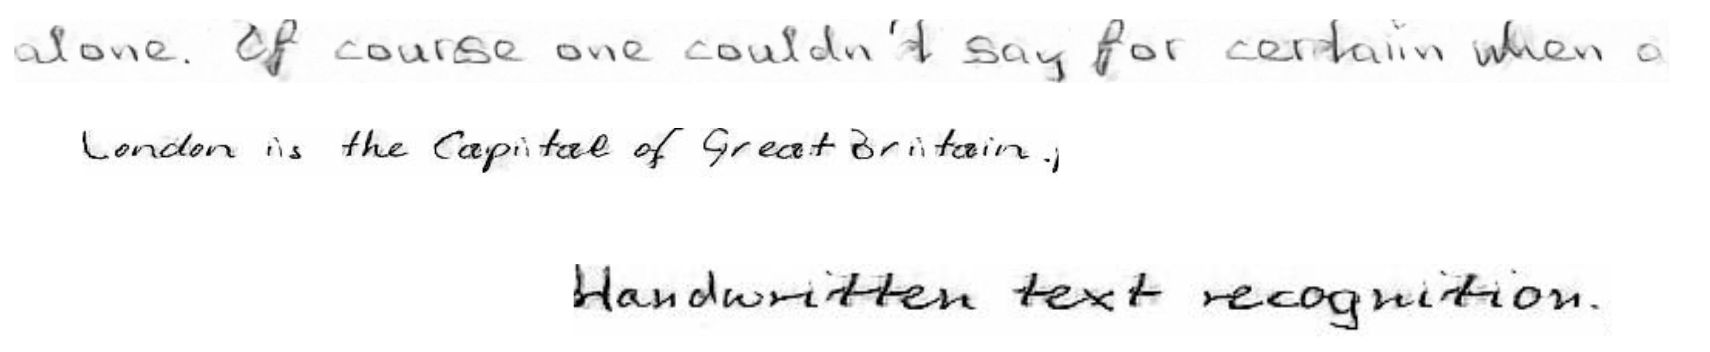
\includegraphics[width=\linewidth]{english_gan.png}
    \end{figure}

    \vspace{5pt}
    RU
    \begin{figure}
        \centering
        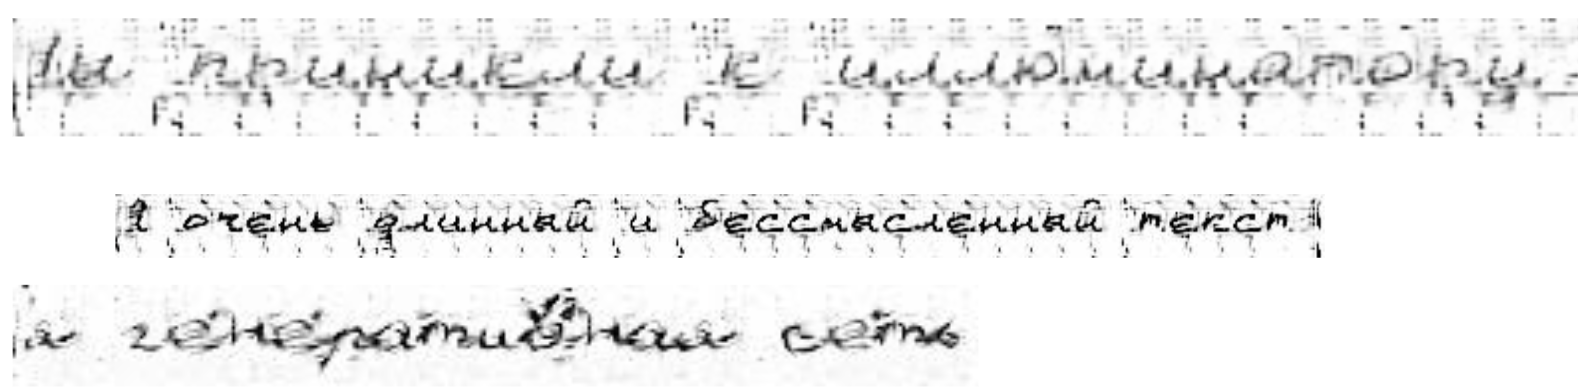
\includegraphics[width=\linewidth]{russian_gan.png}
    \end{figure}
\end{frame}


% \section{Заключение}

\begin{frame}{Заключение}
    \begin{itemize}
        \item Собран большой датасет русских рукописных текстов
        \item Успешно обучена модель распознавания
        \item Применен GAN для генерации русского рукописного текста
    \end{itemize}
\end{frame}

\begin{frame}
    \begin{thebibliography}{9}
        \bibitem{CNN-BGRU}
        Abdallah A., Hamada M., Nurseitov D.
        Attention-based Fully Gated CNN-BGRU for Russian Handwritten Text //Journal of Imaging. – 2020. – Т. 6. – №. 12. – С. 141.

        \bibitem{scrabble_gan}
        Fogel S. et al. Scrabblegan: Semi-supervised varying length handwritten
        text generation //Proceedings of the IEEE/CVF Conference on 
        Computer Vision and Pattern Recognition. – 2020. – С. 4324-4333.

        \bibitem{dan}
        Wang T. et al. Decoupled attention network for text recognition 
        //Proceedings of the AAAI Conference on Artificial Intelligence. – 2020. – Т. 34. – №. 07. – С. 12216-12224.

        \bibitem{chd}
        www.kaggle.com/constantinwerner/cyrillic-handwriting-dataset

        \bibitem{hkr}
        github.com/abdoelsayed2016/HKR\_Dataset

        \bibitem{iam}
        https://fki.tic.heia-fr.ch/databases/iam-handwriting-database

    \end{thebibliography}
\end{frame}

\end{document}